\chapter{Emulators}

Op het moment van schrijven is er slechts één emulator voor de MEGA65,\ \stw{xmega65}; de Xemu-emulatorsuite van LGB. De LGB-ontwikkelaars werken hard om bij te blijven met de ontwikkeling van de MEGA65; niettemin is sommige MEGA65-emulatie mogelijk niet nauwkeurig, maar zou deze voldoende moeten zijn voor softwareontwikkeling op de MEGA65.

% Should there be a link to the LGB suite?

Test software tijdens de ontwikkeling regelmatig op echte hardware, zoals een MEGA65 of een FPGA-board dat een MEGA65-core kan uitvoeren.

Download de broncode van de MEGA65-emulator van \url{https://github.com/lgblgblgb/xemu}.

Download voorgecompileerde versies van \url{https://github.lgb.hu/xemu/}. Installers
zijn beschikbaar voor macOS, Windows en Linux.

Een live ISO-image met de emulator, documentatie en andere hulpprogramma's is beschikbaar via
Forum64.de
op \url{https://www.forum64.de/index.php?thread/104698-xemu-live-system-iso-file/\&postID=1549927\#post1549936}.
Indien u deze wilt gebruiken, vindt u de instructies op bladzijde \pageref{sec:live-iso-image}.

\section{De Xmega65-emulator gebruiken}
\index{emulator}

\subsection{Het toetsenbord}
\label{sec:xemu-keyboard}
\index{toetsenbord}

De MEGA65-toetsenbordindeling is gebaseerd op de Commodore 65, wat afwijkt van een modern pc-toetsenbord. In de meeste gevallen herkent de Xmega65-emulator pc-toetsen als hun equivalente MEGA65-toetsen, zoals letters, cijfers en veelgebruikte modificatietoetsen zoals \specialkey{Shift}. Xmega65 gaat uit van een Amerikaanse (VS-)indeling.

Sommige toetsen komen alleen op het MEGA65-toetsenbord voor en hebben geen pc-equivalenten. Xmega65
gebruikt de pc-toetsen \specialkey{Insert}, \specialkey{Delete}, \specialkey{Home},
\specialkey{End}, \specialkey{Page Up} en \specialkey{Page Down} voor
\megakey{+}, \megakey{\pounds}, \specialkey{CLR\\HOME}, \specialkey{RUN\\STOP},
\specialkey{HELP} en \widekey{RESTORE}, respectievelijk.

\begin{center}
  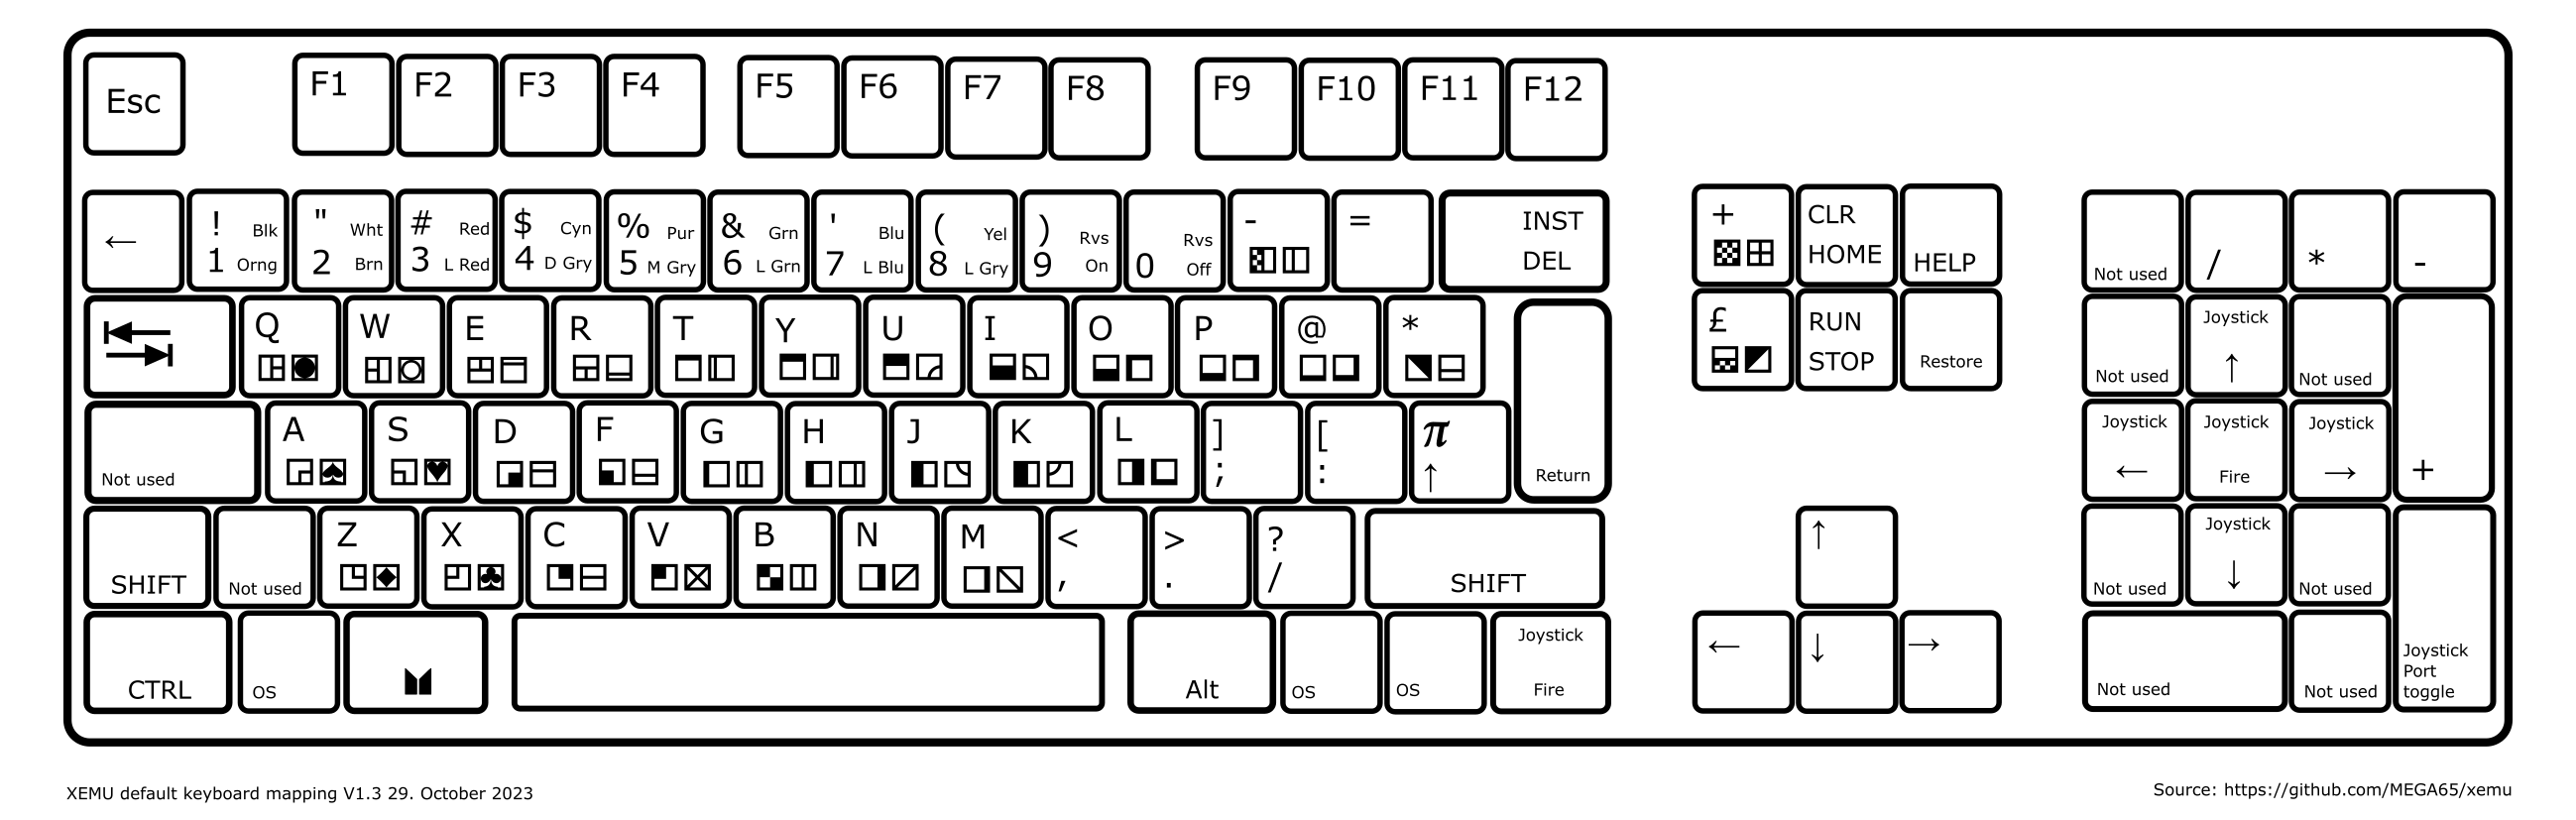
\includegraphics[width=\linewidth]{images/xemu-extended-keyboard.png}
\end{center}

Op de meeste pc-toetsenborden staan \specialkey{RUN\\STOP} en \widekey{RESTORE} naast elkaar,
zodat deze toetscombinatie eenvoudig is in te voeren.

Deze afbeelding toont de PETSCII-glyphen zoals ze op een MEGA65-toetsenbord verschijnen, met de
\megasymbolkey-glyphe links en de \specialkey{Shift}-glyphe rechts. Merk op
dat op een pc-toetsenbord de toets voor \megasymbolkey rechts van de
\specialkey{Shift} staat.

Xemu biedt twee joysticks (een per keer) op het numerieke toetsenbord.
\specialkey{Enter} op het numerieke toetsenbord wordt gebruikt om bij herhaaldelijk drukken poorten 1 en 2 in en uit te schakelen.

Wees u ervan bewust dat de emulator standaard \megakey{F9} \megakey{F10}
\megakey{F11} als eigen sneltoetsen heeft gedefinieerd. Als u deze toetsen wilt gebruiken met de
geëmulieerde MEGA65, moet u de toetsenbordindeling aanpassen. De bestanden staan in de
map met de Xemu-instellingen zoals uitgelegd op bladzijde
\pageref{sec:sdcard-settings-location}. Dit doet u door
\stw{keymap-default.cfg} te kopiëren naar \stw{keymap.cfg} en vervolgens de volgende regels te verwijderen:

\begin{tcolorbox}[colback=black,coltext=white]
\verbatimfont{\codefont}
\begin{verbatim}
XEMU-EXIT F9
XEMU-FULLSCREEN F11
\end{verbatim}
\end{tcolorbox}

en te wijzigen in:

\begin{tcolorbox}[colback=black,coltext=white]
\verbatimfont{\codefont}
\begin{verbatim}
F9 Unknown
F11 Unknown
\end{verbatim}
\end{tcolorbox}

naar:

\begin{tcolorbox}[colback=black,coltext=white]
\verbatimfont{\codefont}
\begin{verbatim}
F9 F9
F11 F11
\end{verbatim}
\end{tcolorbox}

Nadat deze toetsen opnieuw zijn toegewezen, zijn de functies voor volledig scherm en afsluiten nog steeds beschikbaar via
het menu. Klik met rechts (of Ctrl-klik) ergens in het venster om dit te openen.

\subsection{Problemen met starten op Apple MacOS}

Als het bericht \stw{macOS cannot verify that this app is free from malware} verschijnt,
gebruik dan de volgende procedure wanneer u de app voor de eerste keer opent:\index{Apple}
\index{macOS}

\begin{itemize}
  \item Open Finder op uw Mac.
  \item Ctrl-klik (of rechtsklik) op het Xmega65-app-pictogram.
  \item Selecteer in het contextmenu \stw{Open}.
  \item Het bericht verschijnt opnieuw, maar deze keer is er een knop \stw{Open}.
        Klik op \stw{Open}. U hoeft deze procedure slechts de eerste keer uit te voeren.
		Vanaf nu kunt u de app normaal openen.
\end{itemize}

\subsection{Instellingen bijwerken}
\label{sec:sdcard-settings-location}
\index{SD-kaart}

U kunt het Xemu-instellingsbestand bewerken om de toetsenbordindeling aan te passen of een
reservekopie van het SD-kaart-imagebestand te maken. Open vanuit Xemu het menu om deze bestanden te openen: selecteer
menu, selecteer \stw{Debug / Advanced} en vervolgens \stw{Browse system folder}. Bewerk de
bestanden \stw{keymap-default.cfg} en \stw{mega65-default.cfg} met een teksteditor.
Voor specifieke instructies over het wijzigen van \stw{keymap-default.cfg} verwijzen we naar
bladzijde \pageref{sec:xemu-keyboard}.

\begin{center}
  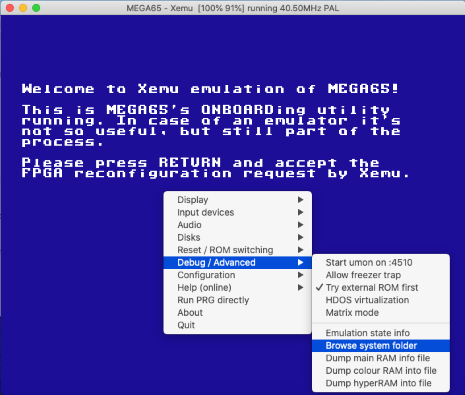
\includegraphics[width=0.5\linewidth]{images/xemusettings.png}
\end{center}

De locatie van de Xemu-systeemmap verschilt per besturingssysteem:

\begin{itemize}
    \item Windows (kan in de adresbalk van de verkenner worden gekopieerd):
    \stw{\%appdata\%$\textbackslash$xemu-lgb$\textbackslash$mega65}
    \item Linux:
    \stw{$\textasciitilde$/.xemu-lgb/}
    \item Macintosh:
    \stw{$\textasciitilde$/Library/Application$\textbackslash$ Support/xemu-lgb/mega65/}
\end{itemize}

\section{De Live ISO-image gebruiken}
\label{sec:live-iso-image}

De Live ISO-image is het product van een vrijwillige gemeenschap; niet van het MEGA65-team. We nemen deze op voor uw gemak.

\subsection{Een opstartbare USB-stick of DVD maken}

Er zijn veel manieren om een live ISO-image te maken. De methode die u kiest hangt af van uw besturingssysteem en of u deze op een USB-station wilt installeren of op een DVD wilt branden. Het branden op een DVD is eenvoudig, ervan uitgaande dat u een computer met een DVD-brander hebt. Als u een sneller opstartbaar USB-station wilt maken, probeert u een van de onderstaande methoden:

Als u Windows gebruikt, overweeg dan een hulpprogramma zoals \url{http://www.isotousb.com/}.

Op Linux kunt u de instructies op \url{https://fossbytes.com/create-bootable-usb-media-from-iso-ubuntu/} volgen.

Voor Apple Macs zijn de instructies op
\url{https://ubuntu.com/tutorials/create-a-usb-stick-on-macos#1-overview} beschikbaar.

Vergelijkbare instructies zijn beschikbaar voor andere populaire computers, zoals Amiga's (\url{https://forum.hyperion-entertainment.com/viewtopic.php?t=3857}) of Sun UltraSPARC-werkstations (\url{https://forums.servethehome.com/index.php?threads/how-to-create-a-bootable-solaris-11-usb.1998/}).

Tot slot is de populaire, eenvoudig te gebruiken en gratis cross-platform belanaEtcher beschikbaar op \url{https://www.balena.io/etcher/}.

\subsection{Aan de slag}

Om potentiële auteursrechtelijke kwesties te vermijden, bevat de opstartbare ISO-image geen propriëtaire ROM's voor de MEGA65, zoals oude C65-ROM's. Het bevat wel een vervangende open-source-ROM van ons OpenROMs-project.\index{OpenROMs} Deze ROM start op in een BASIC 2-omgeving waarmee u veel C64-programma's kunt laden en uitvoeren, zoals te zien is in de onderstaande afbeelding:

\screenshotwrap{images/liveiso-openrom.png}

Als u een C65-ROM met BASIC 10 wilt gebruiken, download het juiste ROM-bestand en plaats het op een andere USB-stick met de naam \stw{MEGA65.ROM}. Bij het opstarten zal de MEGA65 vragen of een ROM is gedownload; zoals te zien is in de onderstaande afbeelding:

\screenshotwrap{images/liveiso-rom-usb-prompt.png}

Als de Live ISO geen ROM kan vinden, zal het u vragen om een ROM te downloaden; zoals hieronder te zien is:

\screenshotwrap{images/liveiso-rom-download-prompt.png}

\subsection{Andere functies van de Live ISO}

Zoals de bovenstaande schermafbeeldingen laten zien, biedt de Live ISO diverse handige bureaubladkortingen. Aan de linkerzijde staan koppelingen om de
MEGA65-emulator en de C65-emulator te starten, zodat u kunt testen of programma's
op beide platforms werken. Zoals eerder vermeld zijn beide emulators in ontwikkeling en mogelijk niet 100\% compatibel.

Een andere koppeling geeft toegang tot het grote Mega65-boek. Deze omvattende band van
ongeveer 800 pagina's bevat de officiële MEGA65-documentatie. Het grootste deel van deze handleiding voor ontwikkelaars is ook opgenomen in het grote Mega65-boek.

Deze ISO bevat ook documentatie voor de C65 Notepad; een programma voor de C65 en MEGA65 geschreven door Snoopy (de ontwikkelaar van de Live ISO-image). Een ``lees mij''-bestand bevat verdere informatie over de Live ISO.

Tot slot zijn er aan de rechterzijde koppelingen om een C65-ROM te downloaden en het grote Mega65-boek bij te werken naar de nieuwste versie. Hiermee voorkomt u dat u steeds een nieuwe opstartbare image moet maken wanneer er een frequente update van het grote Mega65-boek wordt uitgebracht.

De volledige inhoud van de Live ISO-image is toegankelijk via de bestandsverkenner.

% 2022-11-28 edits by nobruinfo
% 2021-03-17 edits by SBC
